\chapter{Chapter 5. Coordinated Analysis}
A coordinated analysis between the magnetosheath and solar wind over $\sim$250 hours was performed in order to compare simultaneous observations. 19 time intervals were identified during these phases for which there were simultaneous measurements by two THEMIS probes, where one was in the solar wind and one was in the magnetosheath. The dayside science and radiation belt science phases of the THEMIS mission offer optimal configuration for direct comparison of the near-Earth solar wind and magnetosphere, specifically the phases in 2008, 2009, 2018, and 2022. MMS was also used in conjunction with the THEMIS probes for the observation intervals identified in 2022. Table \ref{tab:coordinated-observations} in \ref{appendix:observation-periods} shows the subsection of observation intervals for this coordinated analysis. Figure \ref{fig:coordinated-orbits-plot} displays the orbits of THEMIS and MMS during these observation intervals. It should be noted that the data came from simultaneous measurement in two regions during the same interval, \textit{not} a measurement \textit{across} the bow shock.

\begin{figure}
    \centering
    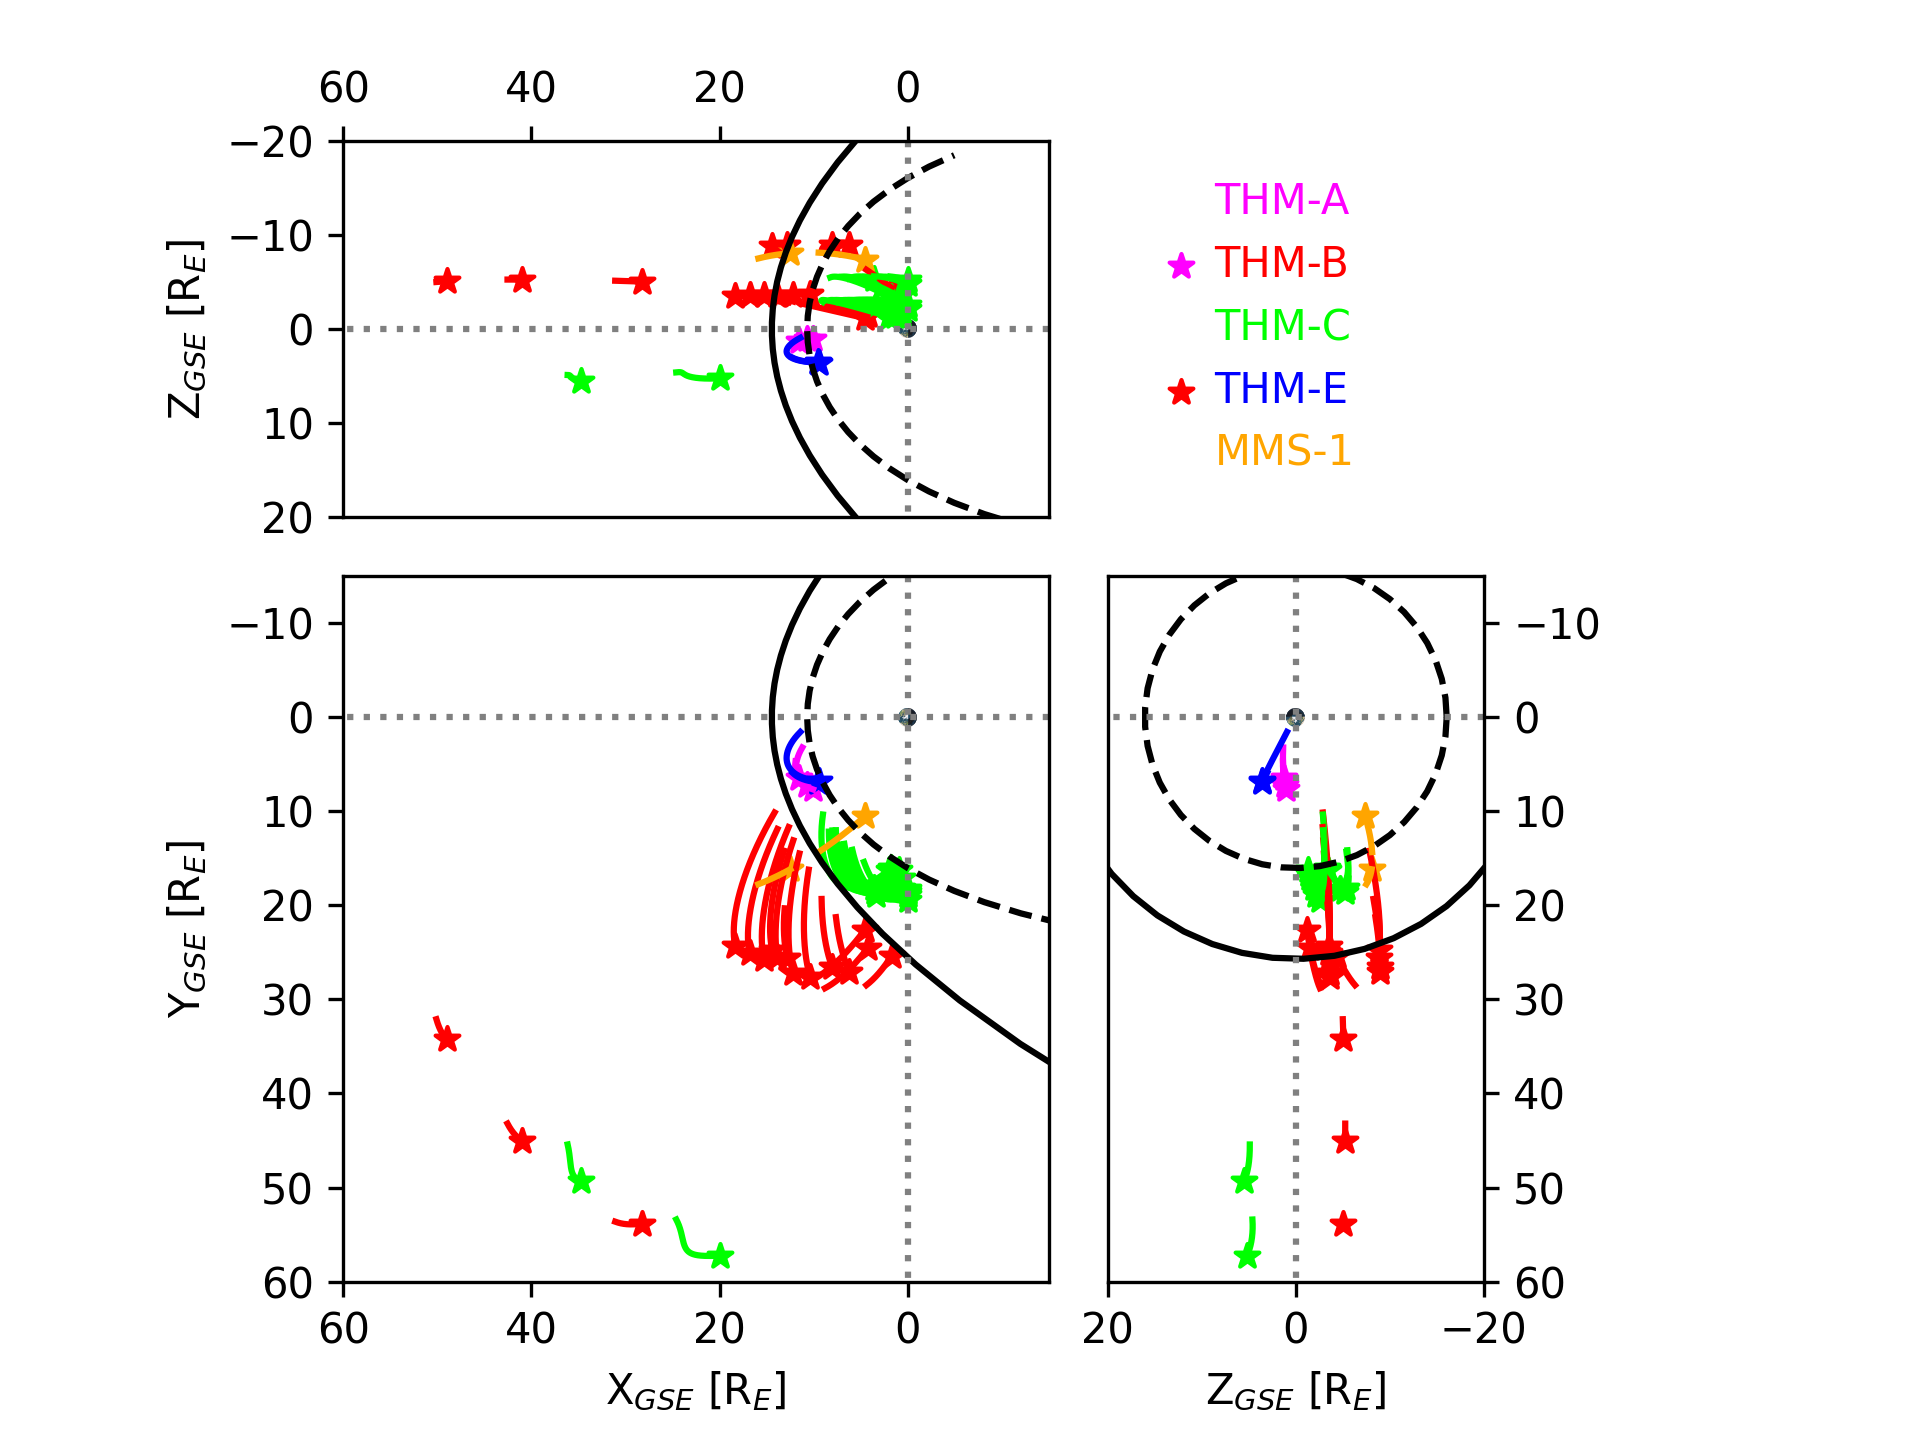
\includegraphics[width=\textwidth]{Figures/Orbits/all_TE_orbits_xy_xz_yz_coordinated.png}
    \caption[Orbits for coordinated observation intervalss]{Orbits for coordinated analysis time periods are shown in the Geocentric Solar Ecliptic (GSE) coordinates for THEMIS probes A, B, C, and E (THM-A, THM-B, THM-C, THM-E) and MMS-1 probe (see legend), with the stars marking the end of each orbit period. The approximate nominal locations of the magnetopause (dashed black line) modeled using the \cite{Shue:1997} model and bow shock (solid black line) modeled using \cite{SlavinHolzer:1984} are shown, based on the IMF data obtained for one period in 2015 only.}
    \label{fig:coordinated-orbits-plot}
\end{figure}

Figure \ref{fig:timeseries-THM-magnetosheath} is an example of one observation such period in the magnetosheath during the coordinated analysis. These measurements were taken in the magnetosheath with THM-C, while the measurements in the solar wind were taken with THM-B (Figure \ref{fig:timeseries-THM-solarwind}). Following the same procedures as outlined in Section \ref{sec:wavelet-algorithm}, 3308 structures were identified in the solar wind, and 3446 structures were identified in the magnetosheath during the coordinated intervals. Table \ref{tab:coordinated-summary} displays the results for the number of events identified with each method. Table \ref{tab:coordinated-MHD-Walen} shows the characterization of the events for each method according to MHD criteria (wavelet analysis) and Wal\'en slope criteria (GS reconstruction).

% Summary table
\begin{table}
    \centering
    \caption{Summary table for events identified via wavelet analysis and the GS reconstruction algorithm during the simultaneous observation intervals.}
    \begin{tabular}{rcccccc}
\hline
Region                    &  Method &  \# Events &  Avg. duration &  Avg. B &  Avg. scale \\
 &    &   &  [mins] &  [nT] &  size [km] \\
\hline
         	         & Wavelet & 1407 & 6.43 & 3.93  & 1.4$\times 10^5$ \\
\textit{Solar wind} 	  & GS 	    & 1901 & 3.46 & 3.90  & 6.0$\times 10^4$ \\
         	           & Total   & 3308 & 4.72 & 3.91  & 9.3$\times 10^4$ \\
\hline
         	         & Wavelet & 1179 & 6.79 & 13.83 & 9.1$\times 10^4$ \\
\textit{Magnetosheath}    & GS      & 2267 & 2.66 & 14.11 & 2.9$\times 10^4$\\
         	         & Total   & 3446 & 4.07 & 14.02 & 5.0$\times 10^4$ \\
\hline
\end{tabular}

    \label{tab:coordinated-summary}
\end{table}

% Combined table (GS + wavelet)
\begin{table}
    \centering
    \caption{Events meeting certain MHD quantity (top) and Wal\'en test slope (bottom) criteria.}
    \begin{tabular}{rrcc}
\hline
& & Solar Wind & Magnetosheath \\
\hline
                  & $|\sigma_m|\geq0.75$                                & 1407 & 1179 \\
\textit{Wavelet}  & $|\sigma_m|\geq0.75, |\sigma_c|\leq0.3$             & 931  & 930 \\
                  & $|\sigma_m|\geq0.75, \sigma_r<0$                    & 1263 & 975 \\
                  & $|\sigma_m|\geq0.75, |\sigma_c|\leq0.3, \sigma_r<0$ & 853  & 836 \\
\hline
                   & Total 		& 1901 & 2267 \\
\textit{GS}        & $|w|\leq 0.3$ & 1777 & 2197 \\
                   & $|w|> 0.3$    & 124  & 70 \\
\hline
\end{tabular}
    \label{tab:coordinated-MHD-Walen}
\end{table}

\noindent It can be seen from Table \ref{tab:coordinated-MHD-Walen} that there were more events characterized as static flux rope structures in the magnetosheath for the coordinated analysis periods. Approximately 79\% of the 1179 structures identified in the magnetosheath using wavelet analysis had a reduced cross helicity magnitude less than 0.3. While there were only incrementally more static structures identified in the magnetosheath than in the solar wind; however, the number of static structures represents a higher percentage of the total number of structures in the magnetosheath versus 66\% in the solar wind. Approximately 97\% of the structures identified in the magnetosheath with the GS reconstruction have a Wal\'en test slope value less than or equal to 0.3 for the coordinated event lists. In the solar wind, the percentage is slightly lower at 93\%, despite the number of structures identified with $|w|\leq 0.3$ being over 400 less than the number of structures in the magnetosheath.

The wavelet analysis results for the coordinated periods are complimentary to the extended analysis periods, with a larger percentage of structures being identified as static structures in the magnetosheath than in the solar wind. However, in the extended analysis, there was a much smaller difference ($\sim$1\%) between the two regions. Additionally, there were more structures with $|w|\leq 0.3$ in the solar wind than in the magnetosheath for the extended analysis, which differs from the coordinated analysis. Figures \ref{fig:histogram-duration-coordinated} through \ref{fig:histogram-Asplit-coordinated} show the distributions of selected parameters from events identified during the coordinated intervals.

\begin{figure}
    \centering
    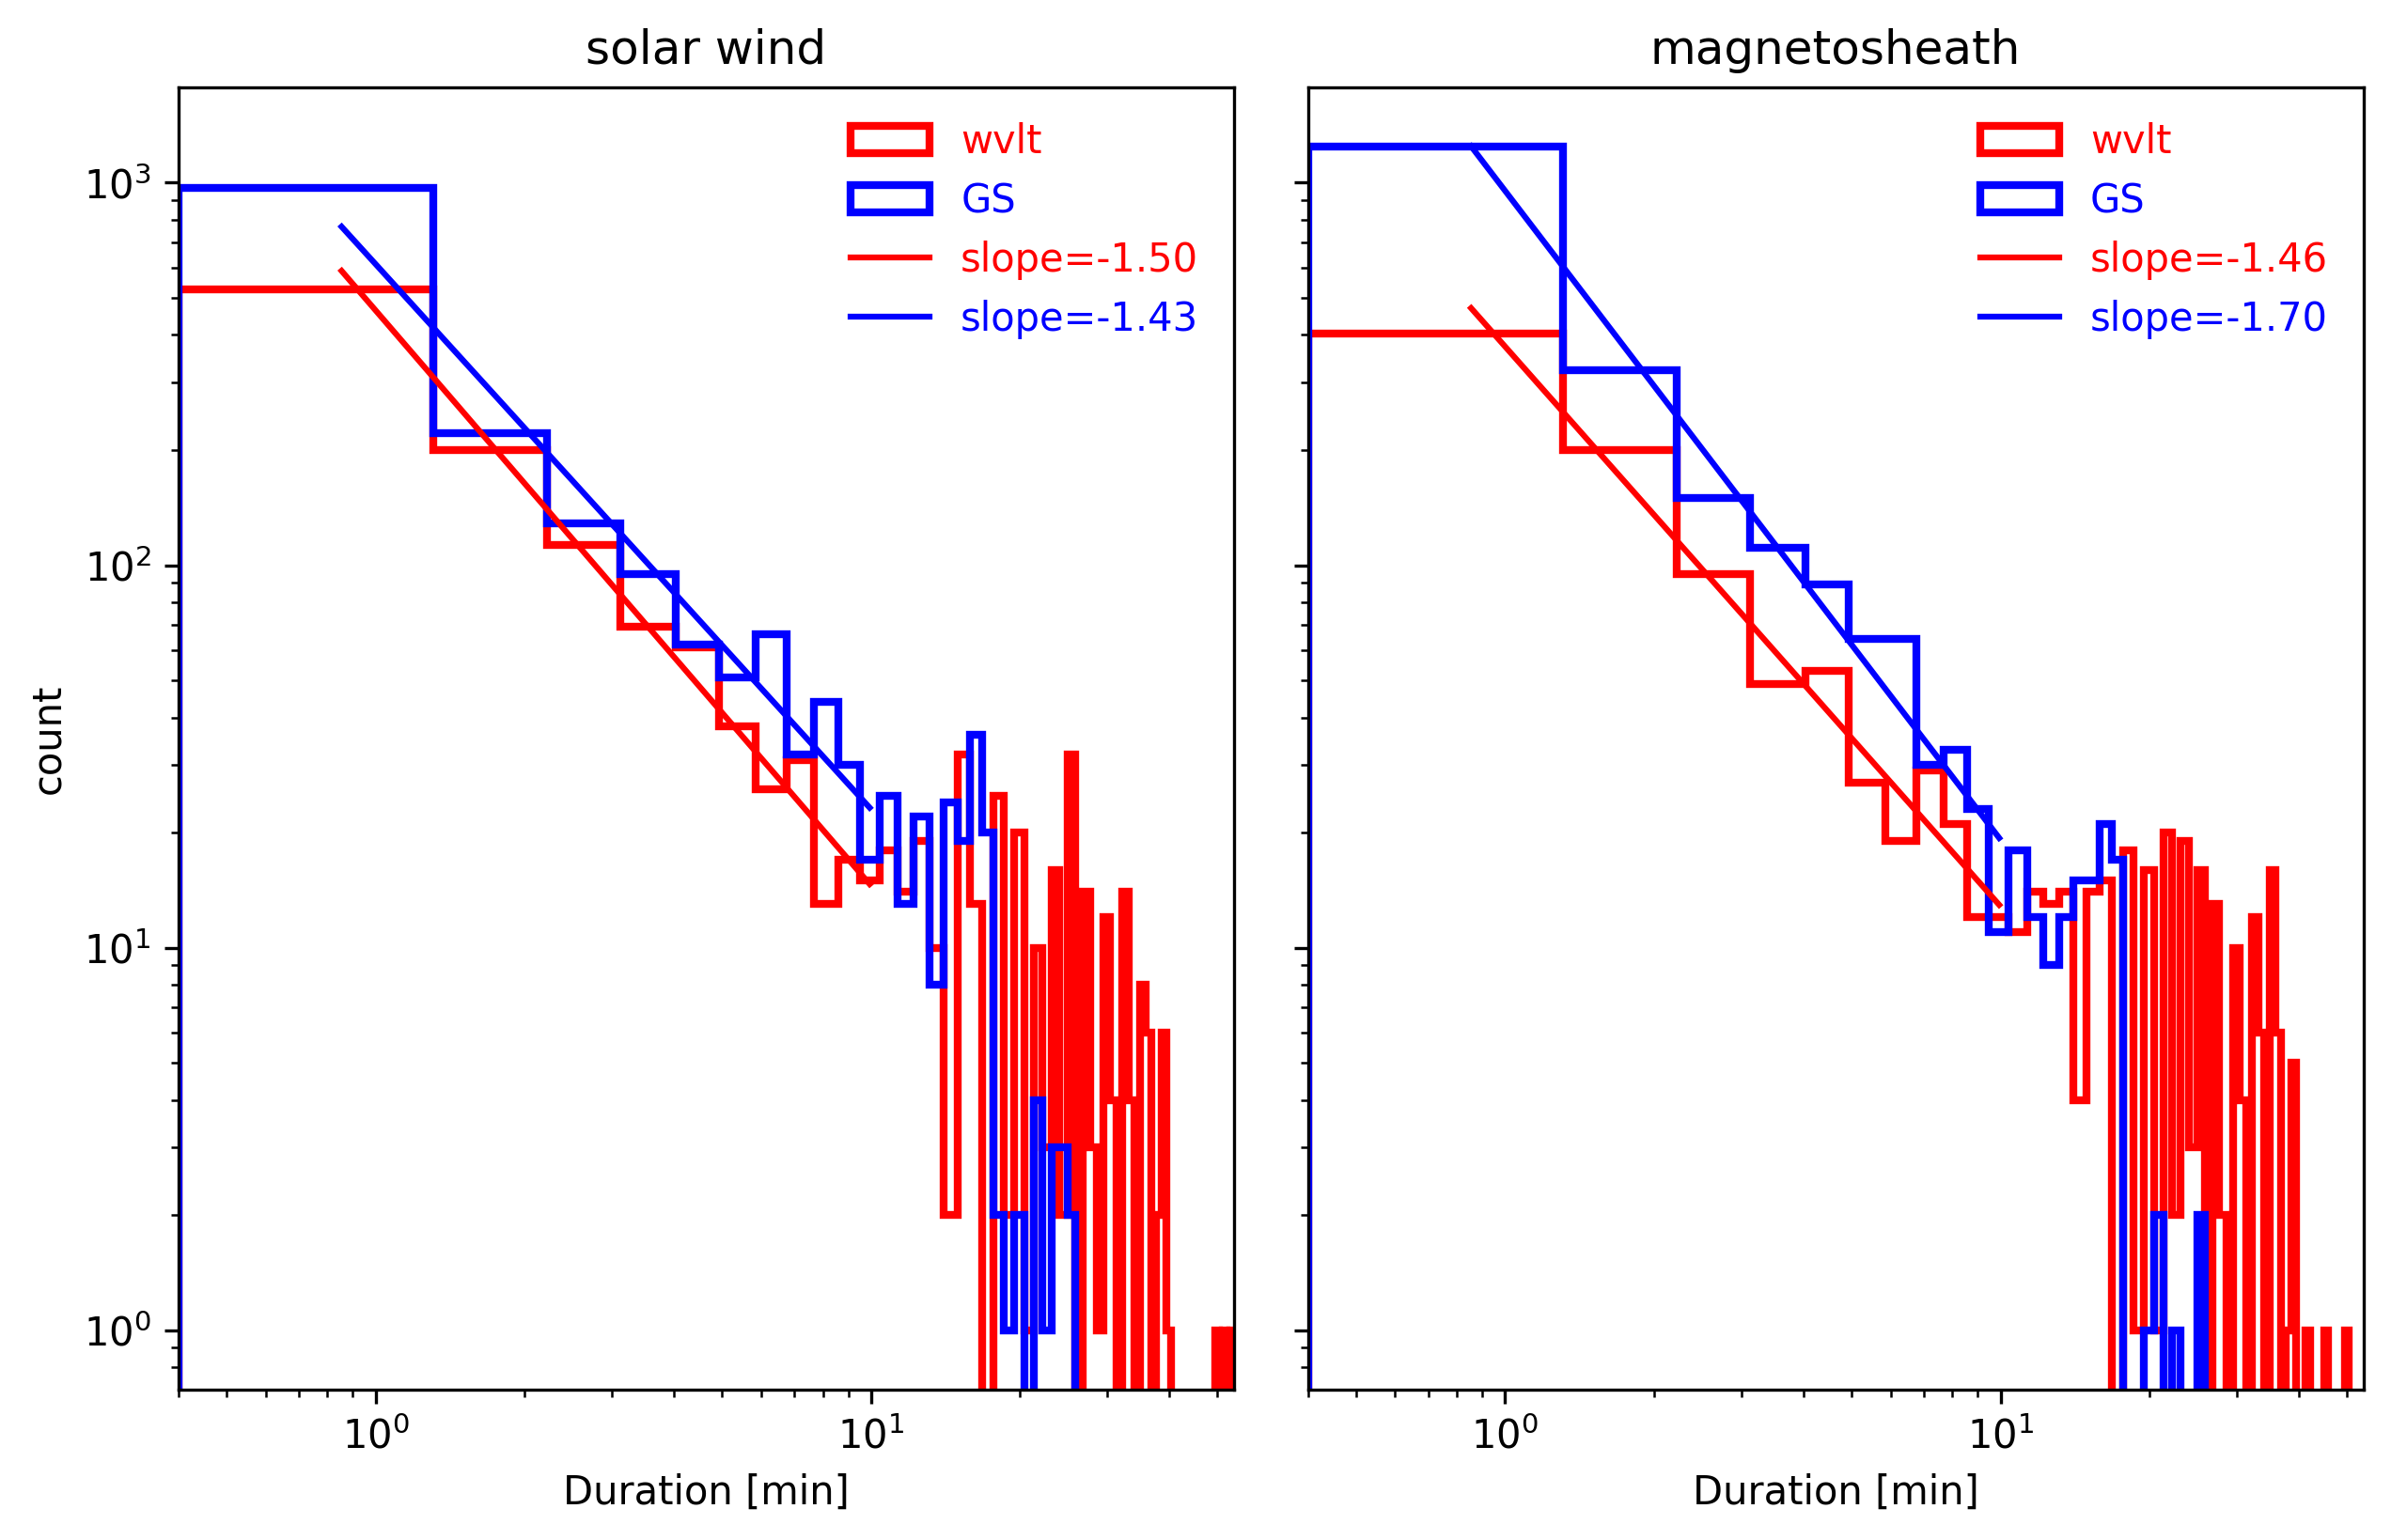
\includegraphics[width=\textwidth]{Figures/Histograms/duration_coordinated.png}
    \caption[Histogram of duration from coordinated analysis]{Histogram of the duration of events identified (during the coordinated orbit intervals) by using wavelet analysis (red lines) and the GS reconstruction method (blue lines).}
    \label{fig:histogram-duration-coordinated}
\end{figure}

\begin{figure}
    \centering
    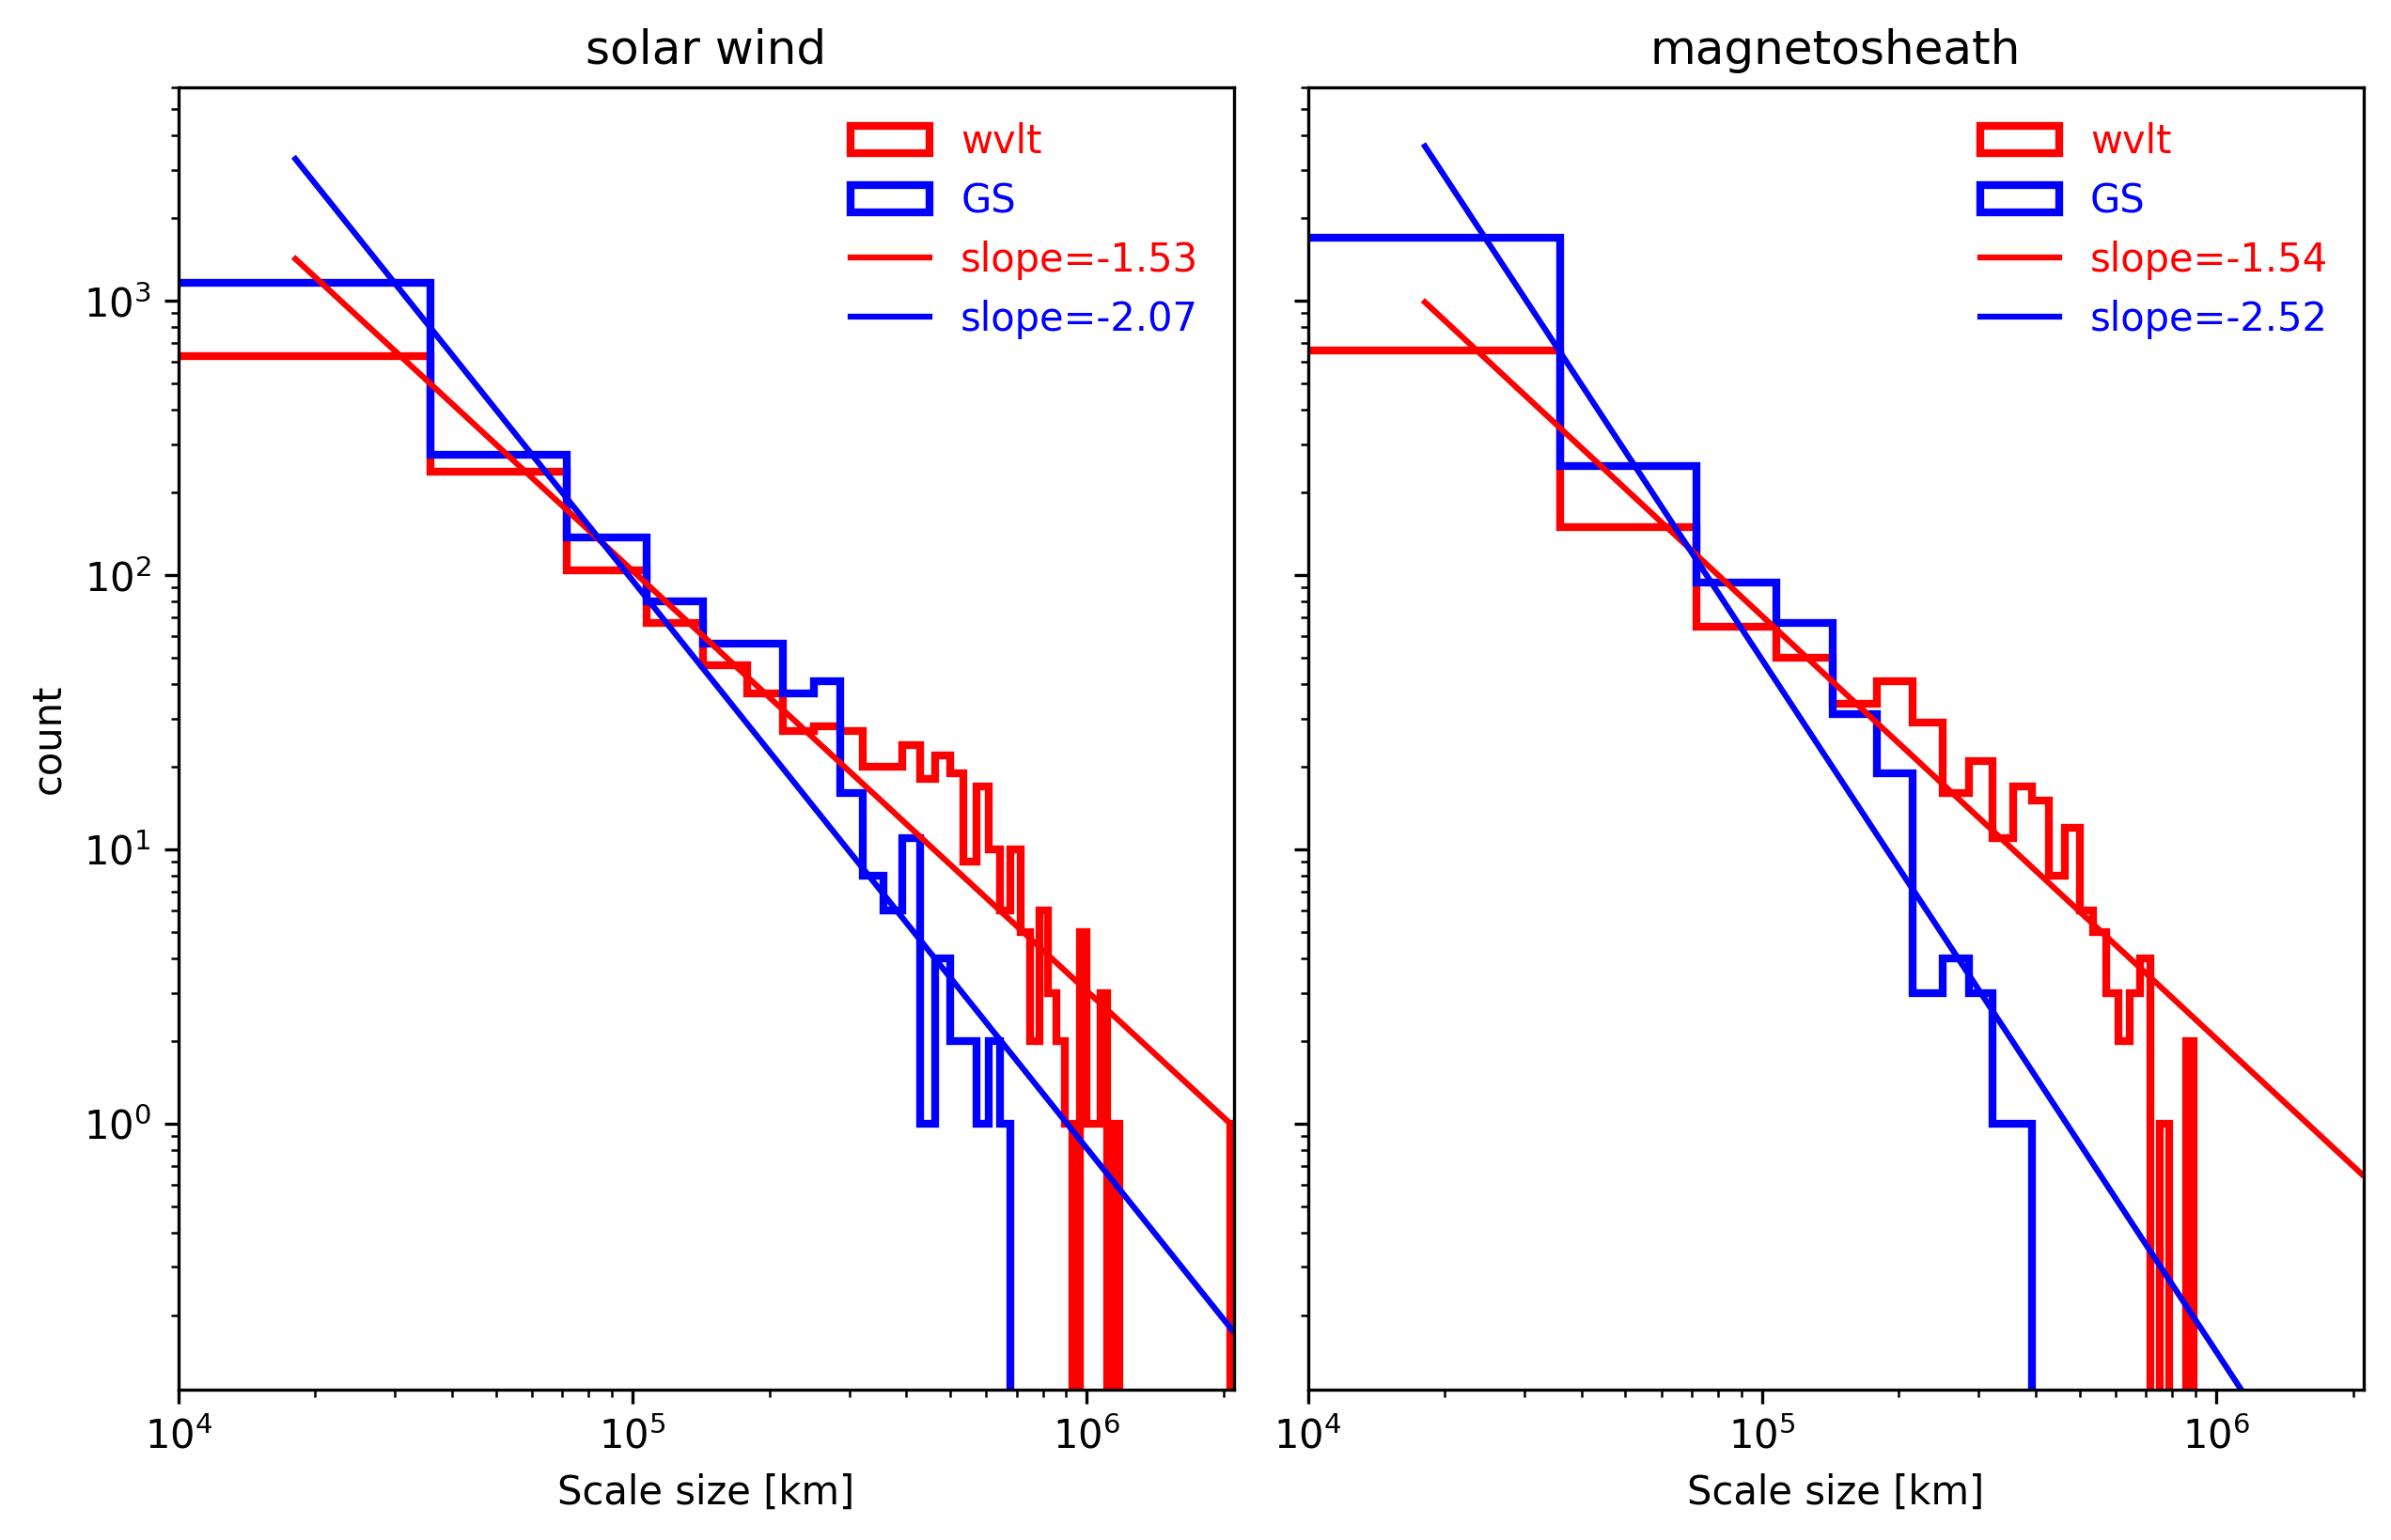
\includegraphics[width=\textwidth]{Figures/Histograms/scalesize_coordinated.png}
    \caption[Histogram of scale size from coordinated analysis]{Same as Figure \ref{fig:histogram-duration-coordinated} but for scale size of events identified during the coordinated orbit intervals.}
    \label{fig:histogram-scalesize-coordinated}
\end{figure}

\begin{figure}
    \centering
    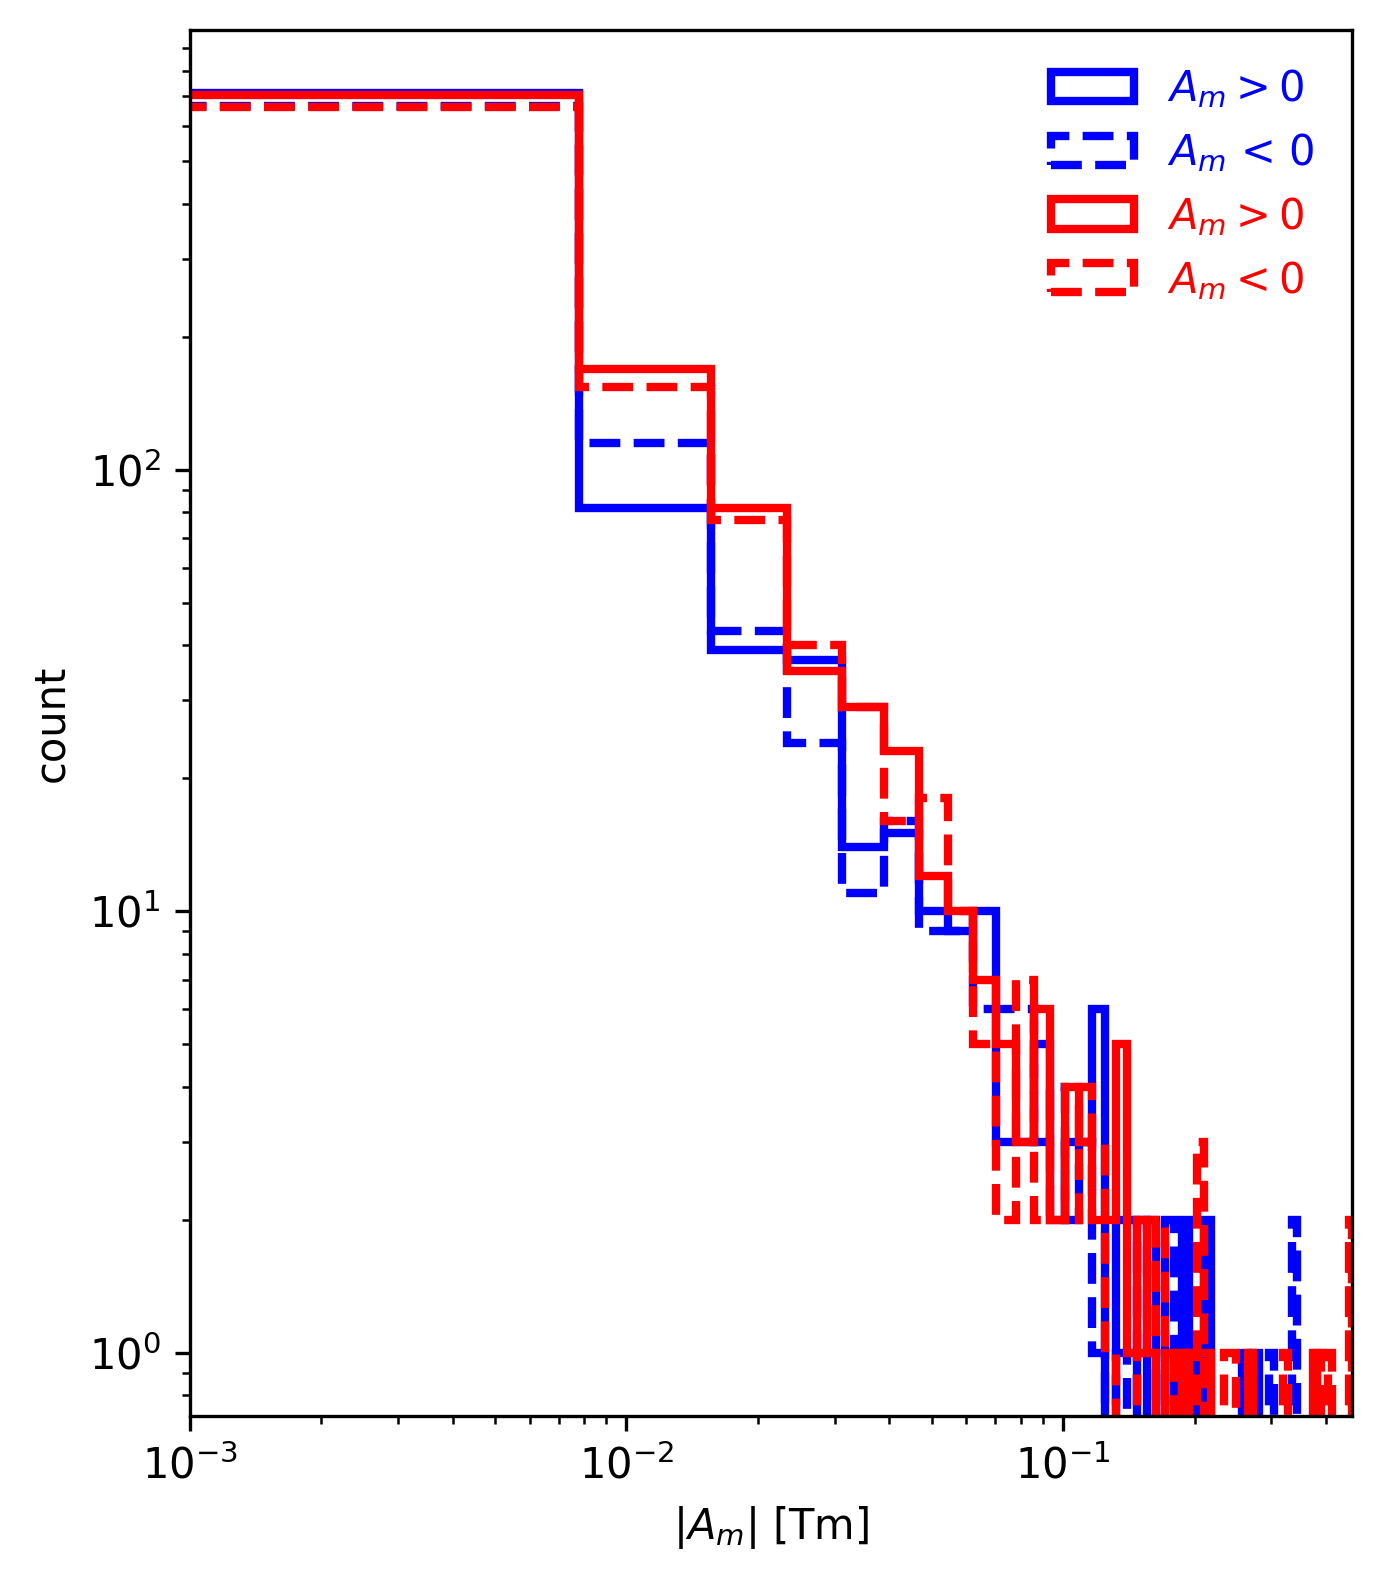
\includegraphics[width=0.7\textwidth]{Figures/Histograms/Asplit_coordinated.png}
    \caption[Histogram of poloidal magnetic flux per unit length from coordinated analysis]{Histograms for the local maximum magnetic flux $|A_m|$ of events identified via GS analysis during the coordinated orbit intervals.}
    \label{fig:histogram-Asplit-coordinated}
\end{figure}


% Figure \ref{fig:mhd-over-time} displays the reduced magnetic helicity $\sigma_m$ and reduced cross helicity $\sigma_c$ as calculated by equations \ref{eq:sigm} and \ref{eq:sigc}, over time. At each data point in time, $\sigma_m$ and $\sigma_c$ were averaged over the scales.

% \begin{figure}
%     \centering
%     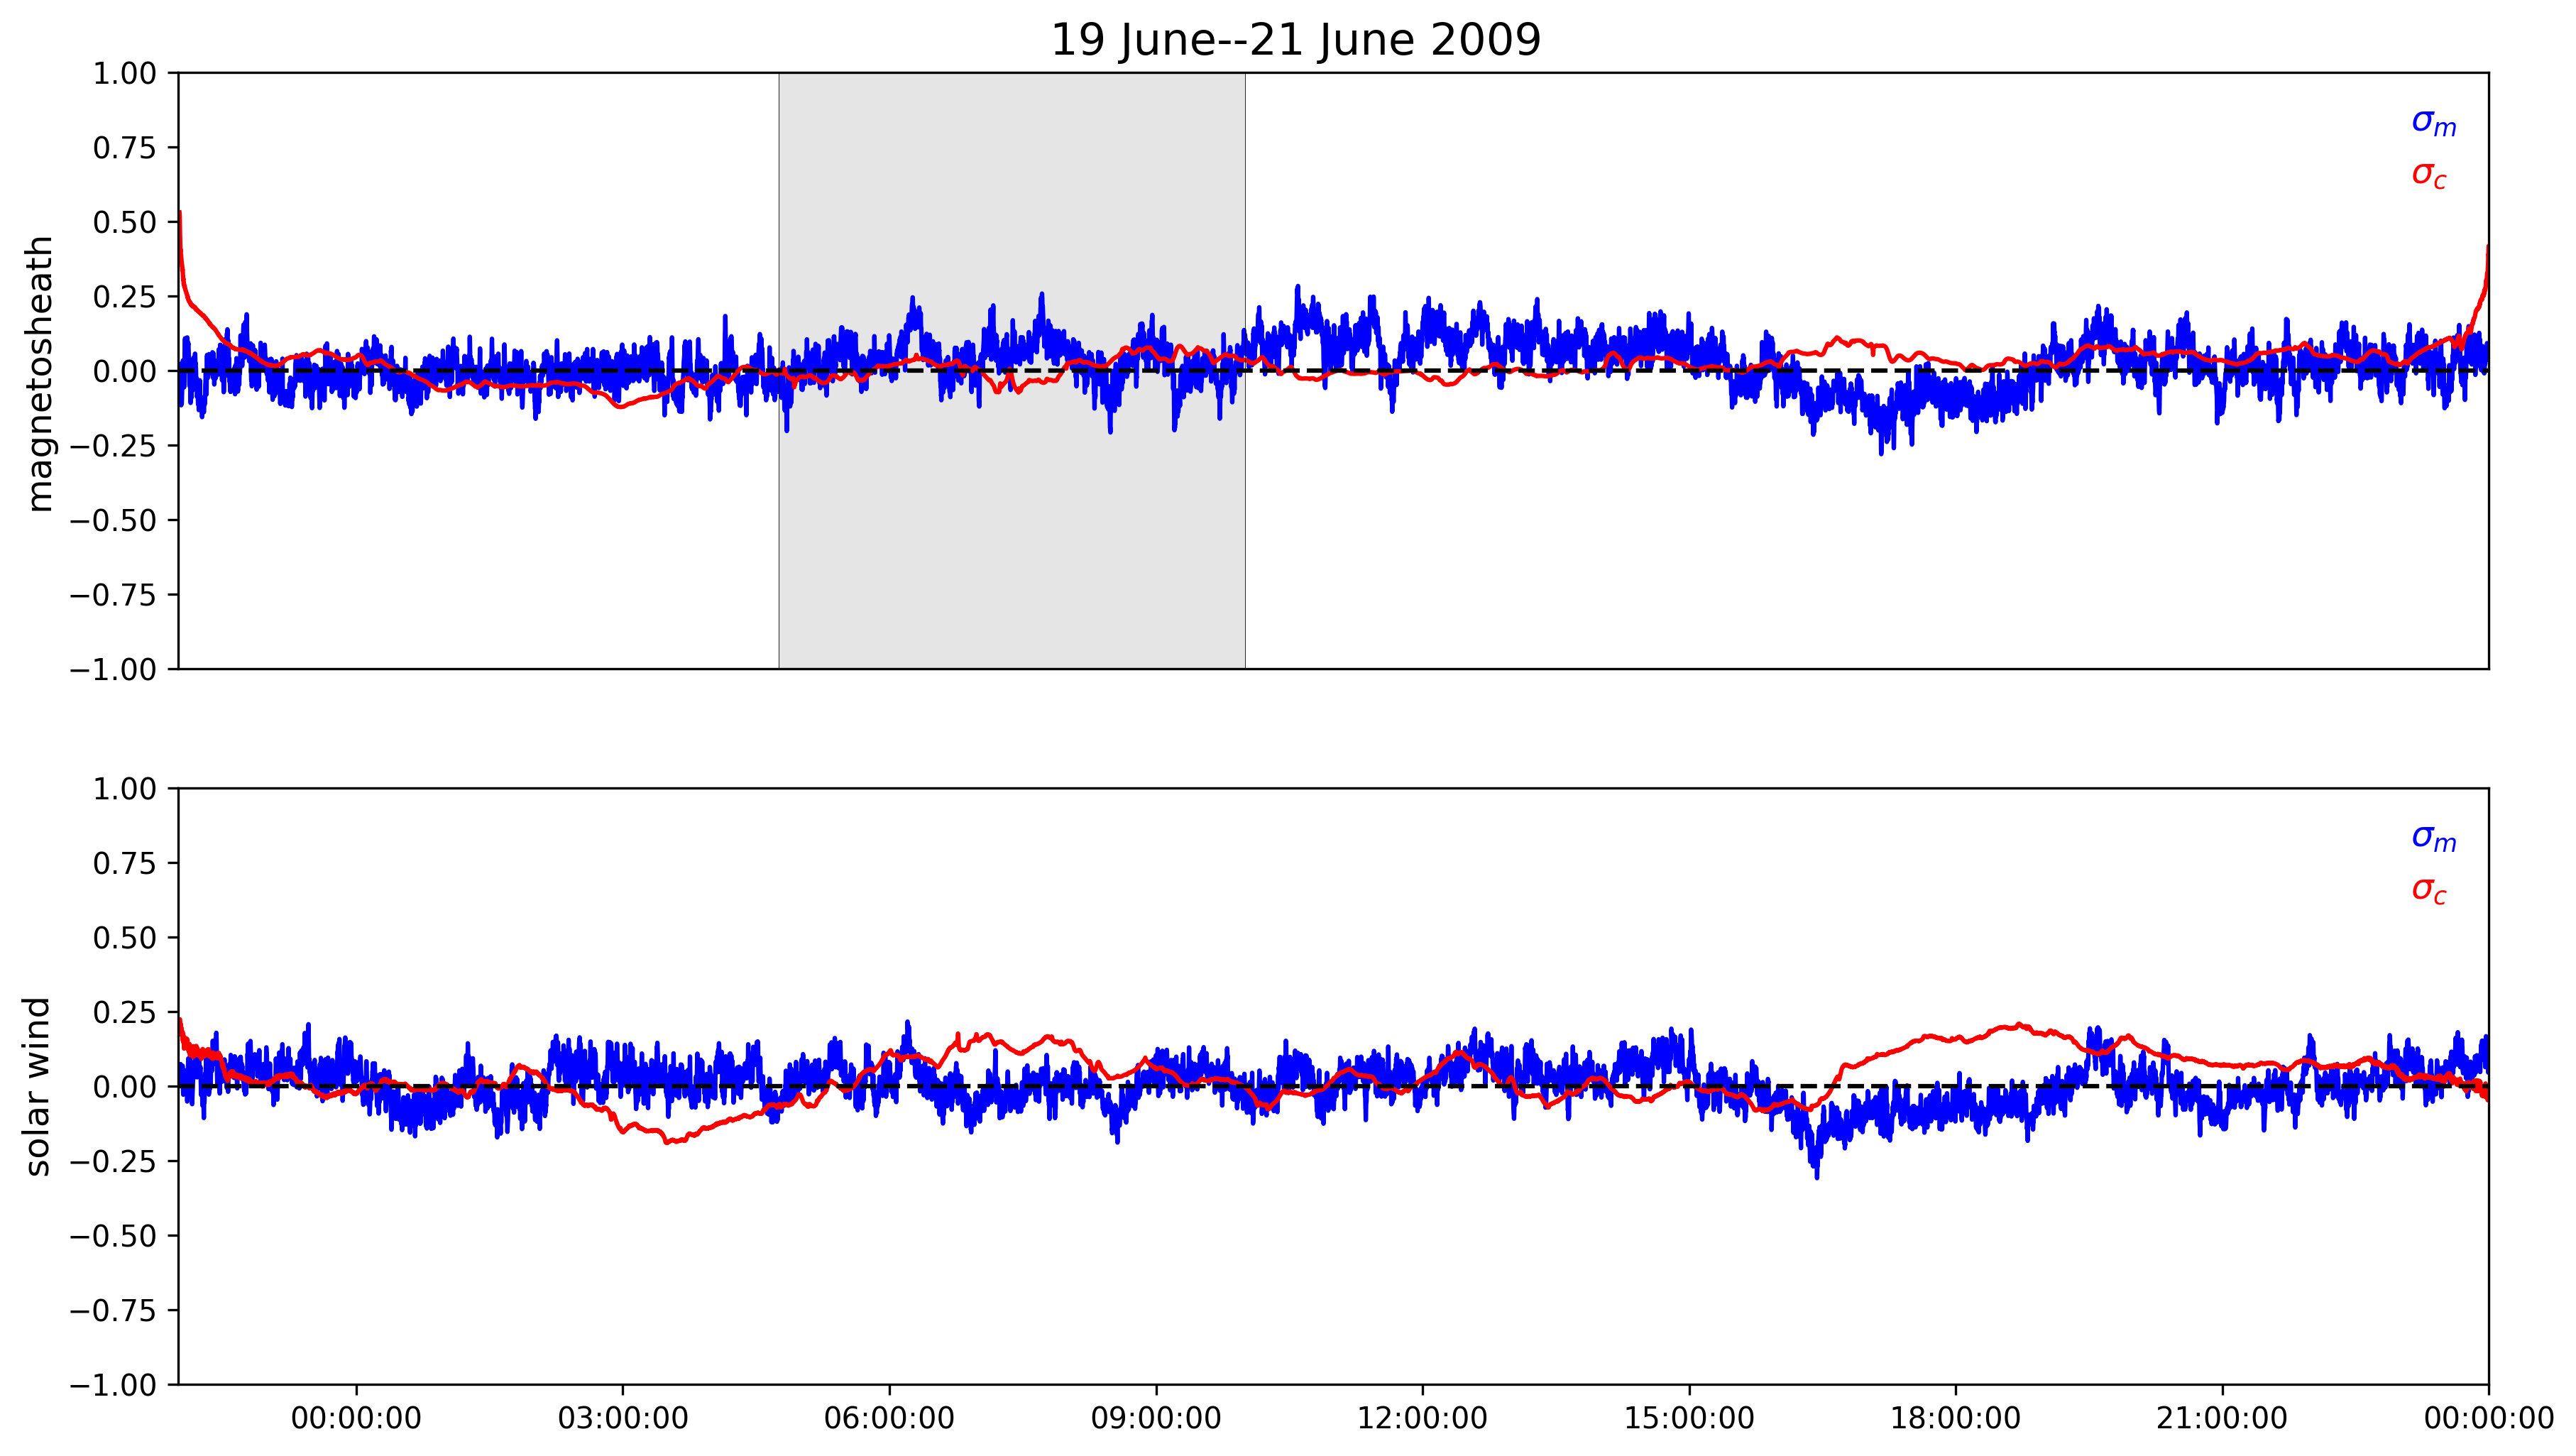
\includegraphics[width=\linewidth]{Figures/sigm_sigc_coordinated_20090619_20090621.png}
%     \caption[Scale-averaged reduced magnetic helicity and reduced cross helicity over time for 19-21 June 2009]{The scale-averaged reduced magnetic helicity $\sigma_m$ and reduced cross helicity $\sigma_c$ as calculated by the wavelet analysis method (equations \ref{eq:sigm} and \ref{eq:sigc}) over one observation period by THM-C in the magnetosheath (top) and THM-B in the solar wind (bottom) over 19-21 June 2009. The grey interval in the top panel represents a bow shock crossing from which observations are removed in this study.}
%     \label{fig:mhd-over-time}
% \end{figure}